% ------------------------------------------------------------------------ %
% !TEX encoding = UTF-8
% !TEX TS-program = pdflatex
% !TEX spellcheck = en-EN
% ------------------------------------------------------------------------ %
%
% ------------------------------------------------------------------------ %
% 	                            FRONTISPIECE
% ------------------------------------------------------------------------ %
%
% Document type
\documentclass[a4paper,12pt,twoside]{report}
%
% Languages setup
\usepackage[italian,english]{babel}
%
% Margins setup
\usepackage[margin=20mm,top=40mm]{geometry}
%
% Packages to include...
\usepackage{hyperref}
%
% Mathematical symbols
\usepackage{amsmath}
%
% Various symbols
\usepackage{textcomp}
\usepackage[mathscr]{euscript}
%
% Figures
\usepackage{epsfig}
\usepackage{graphicx}
\usepackage{xcolor}
\usepackage{subfigure}
%
% Headers
\usepackage{fancyhdr}
%
% Characters encoding
\usepackage[ansinew]{inputenc}
\usepackage[OT1]{fontenc}
%
% Page style
\fancyhead[L]{\chaptername \thechapter}
\fancyhead[LO]{\thesection} \fancyhead[RO]{\sectionmark}
\lhead{\slshape Ch. \thechapter}
%
%%%%%%%%%%%%%%%%%%%%%%%%%%%%%%%%%%%%%%%%%%%%%%%%%%%%%%%%%%%%%%%%%%%%%
%                      Start of the document                        %
%%%%%%%%%%%%%%%%%%%%%%%%%%%%%%%%%%%%%%%%%%%%%%%%%%%%%%%%%%%%%%%%%%%%%


\begin{document}


% Start of the frontispiece

\thispagestyle{empty}
\enlargethispage{40mm}
\begin{center}
\Large{\textsc{Politecnico di Milano}}\\
\begin{figure}[h]
\begin{center}
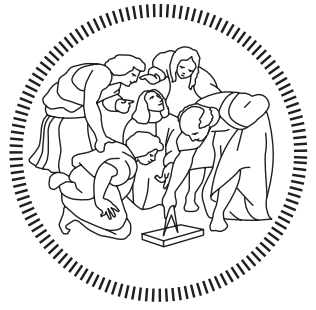
\includegraphics[scale=0.25]{images/logoPolimi.png}
\end{center}
\end{figure}
\vspace{-8mm}
\large{Corso di Laurea Magistrale in Computer Science and Engineering}\\
\large{Dipartimento di Elettronica e Informazione}\\
\vspace{15mm}

\begin{center}
\noindent\rule{17cm}{0.4pt}
\end{center}

% Project title
\vspace{1mm}
{\textbf{\Huge{Usability Study Report}}} \\
\vspace{5mm}
{\textbf{\textit{\Large{The Big Family}}}} \\
\noindent\rule{17cm}{0.4pt}

\vspace{10mm}

{\Large{\textit{Hypermedia Applications 2018 Project}}}


% authors
\begin{center}
\vspace{10mm}
Authors:
\vspace{-3mm}
\end{center}
\begin{center}
\begin{tabular}{l l }
Alessandro Aimi \href{mailto:alessandro.aimi@mail.polimi.it}{alessandro.aimi@mail.polimi.it}  \\
Roberto Bigazzi \href{mailto:roberto.bigazzi@mail.polimi.it}{roberto.bigazzi@mail.polimi.it}
\end{tabular}
\end{center}

% abstract
\begin{center}
\vspace{10mm}
Abstract:
\vspace{-4mm}
\end{center}
\end{center}
\large{This document is a report for the usability of ``The Big Family" site hosted on \href{https://polimi-hyp-2018-team-10483610.herokuapp.com}{https://polimi-hyp-2018-team-10483610.herokuapp.com} developed for Hypermedia Application course project. User testing is used for the purpose. Evaluation is done on content, navigation, and interface design (semiotics, cognitive, graphics).}
\vspace{10mm}


% date
\begin{center}
\vspace{-4mm}
\it{\large{16/05/2018}}
\end{center}
\begin{center}
\vspace{-4mm}
{\large{Academic Year 2017-2018}}
\end{center}

% End of the frontispiece
% End of the document

\end{document}